\documentclass{article}
\usepackage{booktabs}
\usepackage{pgfplots}
\usepackage{amsmath}
\begin{document}
\title{CUDA Bitonic Sort Optimization}
\author{}
\date{}
\maketitle

\section{Overview}
This report summarizes timing results for a baseline bitonic sort implementation and three optimizations. The baseline source is \texttt{bitonic\_sort.cu} and the modifications are \texttt{mod1.cu}, \texttt{mod2.cu}, and \texttt{mod3.cu}.

All timings measure kernel execution using the CUDA synchronization approach described in the assignment. The array size was $2^{30}$ values and all tests were compiled for a compute capability 8.6 device.

\section{Results}
The baseline kernel required 3501.20~ms. Table~\ref{tab:times} lists the measured times and speedup relative to the baseline. Speedup is computed as $T_{\text{baseline}}/T_{\text{mod}}$.

\begin{table}[h]
\centering
\begin{tabular}{lrr}
\toprule
Kernel & Time (ms) & Speedup \\ \midrule
Baseline & 3501.20 & 1.00 \\
Modification~1 & 3497.79 & 1.00 \\
Modification~2 & 1977.88 & 1.77 \\
Modification~3 & 1749.70 & 2.00 \\ \bottomrule
\end{tabular}
\caption{Kernel execution times for sorting $2^{30}$ values and speedup over the baseline.}
\label{tab:times}
\end{table}

Figure~\ref{fig:speedup} visualizes the speedup achieved by each optimization.

\begin{figure}[h]
\centering
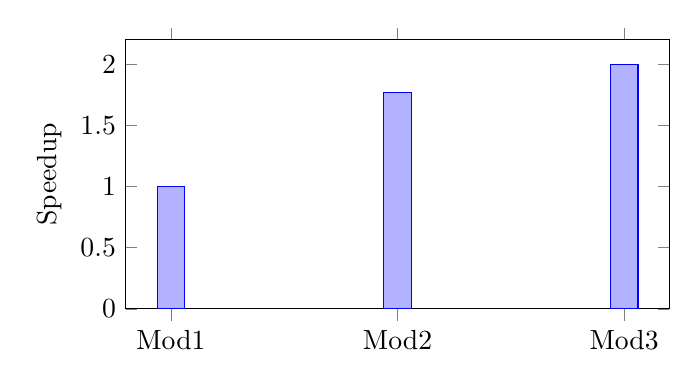
\begin{tikzpicture}
\begin{axis}[
    ybar,
    symbolic x coords={Mod1,Mod2,Mod3},
    xtick=data,
    ylabel={Speedup},
    ymin=0,ymax=2.2,
    width=0.7\linewidth,
    height=5cm
]
\addplot coordinates {(Mod1,1.00) (Mod2,1.77) (Mod3,2.00)};
\end{axis}
\end{tikzpicture}
\caption{Speedup relative to the baseline implementation.}
\label{fig:speedup}
\end{figure}

\section{Discussion}
\textbf{Modification~1} eliminates idle threads by having every CUDA thread operate on exactly one pair of indices.\par
\textbf{Modification~2} merges multiple minor steps into a single kernel when possible, reducing kernel launch overhead.\par
\textbf{Modification~3} builds on the merged-kernel approach by keeping the j/set loop inside the kernel while each thread processes multiple index pairs to increase cache reuse. In these tests each thread handled four pairs.

\end{document}
